\section{Exploring Bivariate Relationships in R}


Let's use a dataset called |iris| (included in the standard R distribution) to explore bivariate relationships between variables. This data set was made famous by R. A. Fisher who used it to illustrate many of the fundamental statistical methods he developed. The data set consists of four morphometric measurements for specimens from three different iris species. Use the R help to read about the iris data set (\lstinline!?iris!). We'll be using this data set repeatedly in future weeks so familiarize yourself with it.
%
\begin{R}
> ?iris
> names(iris)
[1] "Sepal.Length" "Sepal.Width"  "Petal.Length" "Petal.Width"
[5] "Species"
> unique(iris$Species)
[1] setosa     versicolor virginica
Levels: setosa versicolor virginica
> dim(iris)
[1] 150   5
\end{R}

For now let's just work with the \Species{I.~setosa} specimens. Read the help file for |subset()|.
\begin{R}
> setosa <- subset(iris, Species == 'setosa', select = -Species)
> dim(setosa)
[1] 50  4
> names(setosa)
[1] "Sepal.Length" "Sepal.Width"  "Petal.Length" "Petal.Width"
\end{R}
Notice how we used the |select| argument to |subset()| in order to drop the Species column. Let's explore the setosa subset with some graphs.
%
\begin{R}
> plot(setosa$Sepal.Length, setosa$Sepal.Width)
> plot(setosa$Sepal.Width ~ setosa$Sepal.Length)
\end{R}
Did you notice what is different between the two versions above? You can
also use the \lstinline!data! argument with plot, like so:
\begin{R}
> plot(Sepal.Width ~ Sepal.Length, data = setosa)
\end{R}
The \lstinline!xyplot()! function from the \lstinline!lattice! package
does pretty much the same thing:
%
\begin{R}
> library(lattice)
> xyplot(Sepal.Width ~ Sepal.Length, data = setosa)
\end{R}

Let's also explore a number of the other bivariate relationships in this data set:
%
\begin{R}
# an alternate way to generate such a plot, using the data argument to specify where the variables are defined
> plot(Petal.Length ~ Sepal.Length, data = setosa)

# same form as the first plot, but changing the character used for the plot using the 'pch' argument. The 'cex' argument increases the size of the characters by the specified factor (1.5x in this case)
> plot(setosa$Sepal.Length, setosa$Petal.Width, pch = 20, cex=1.5)
\end{R}

Often times it's useful to look at many bivariate relationships simultaneously. The |pairs()| function allows you to do this:
%
\begin{R}
> pairs(setosa)
\end{R}
%
\begin{figure}[htbp]
\centering
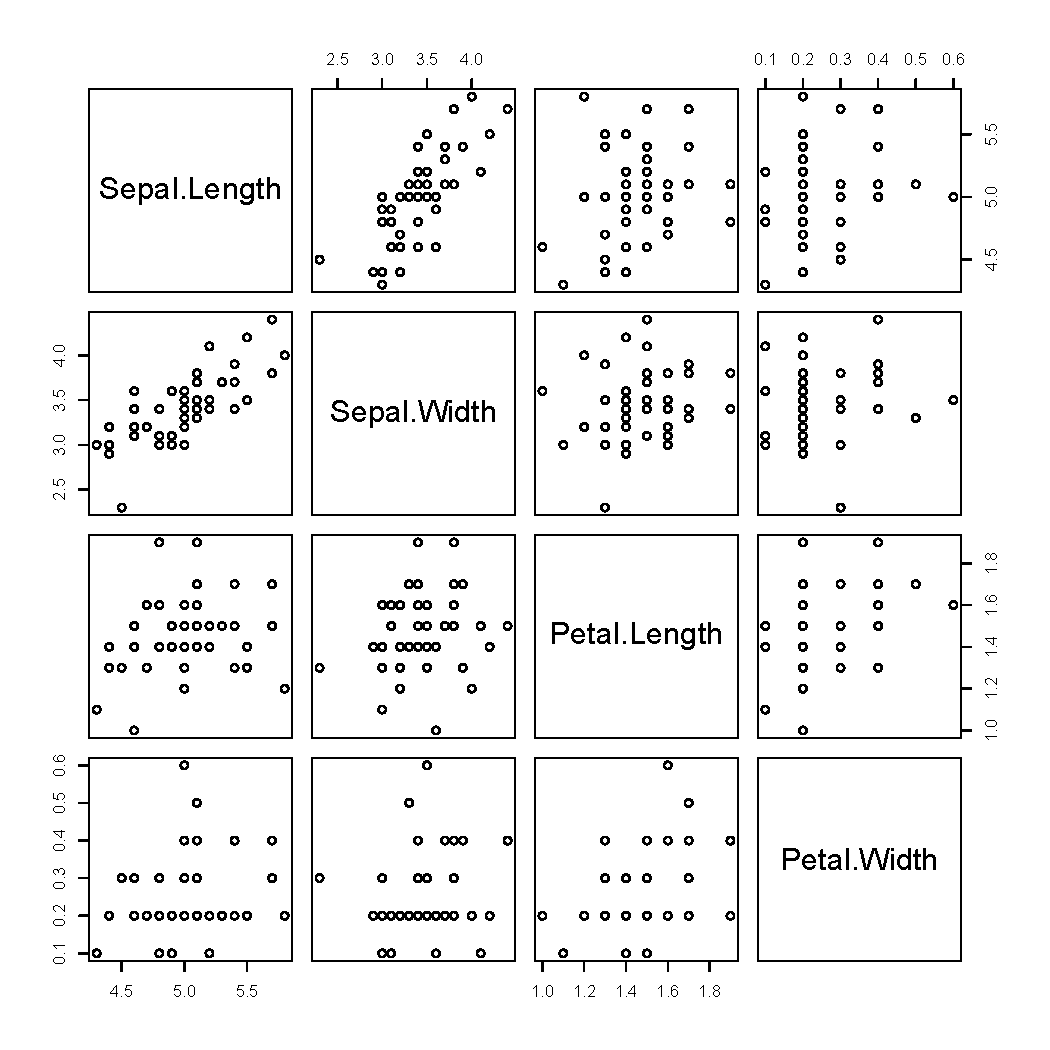
\includegraphics[width=0.5\columnwidth]{./figures/hands-on2/pairs-output.pdf}
\caption{Output of the \lstinline!pairs()! function for the \Species{I.~setosa} specimens in the \lstinline|iris| dataset.}
\end{figure}

Let's return to our use of the dot product to explore the relationship between variables. First let's add a function to |vecgeom.R| to calculate the cosine of the angle between to vectors.
\begin{R}
# add to vecgeom.R

vec.cos <- function(x,y) {
  # Calculate the cos of the angle between vectors x and y
  len.x <- veclength(x)
  len.y <- veclength(y)
  return( (x %*% y)/(len.x * len.y) )
}
\end{R}
We can then use this function to examine the relationships between the variables in the setosa dataset. First we'll center the setosa dataset using the |scale()| function. |scale()| has two logical arguments |center| and |scale|. By default both are |TRUE| which will center \emph{and} scale the variables. But for now we just want to center the data. |scale()| returns a matrix object sow we use the |data.frame| function to cast the object back to a data frame.
\begin{R}
> source("/Users/pmagwene/Downloads/vecgeom.R")
> ctrd <- scale(setosa,center=T,scale=F)
> class(ctrd)
[1] "matrix"
> names(ctrd)
NULL
> ctrd <- data.frame(scale(setosa,center=T,scale=F))
> class(ctrd)
[1] "data.frame"
> names(ctrd)
[1] "Sepal.Length" "Sepal.Width"  "Petal.Length" "Petal.Width"
> vec.cos(ctrd$Sepal.Length, ctrd$Sepal.Width)
          [,1]
[1,] 0.7425467
> vec.cos(ctrd$Sepal.Length, ctrd$Petal.Length)
          [,1]
[1,] 0.2671758
> vec.cos(ctrd$Sepal.Length, ctrd$Petal.Width)
          [,1]
[1,] 0.2780984
\end{R}

Consider the values above in the context of the scatter plots you generated with the |pairs()| function; and then recall that for mean-centered variables, $\mathsf{cor}(X,Y) = r_{XY} = \cos \theta = \frac{\vec{x} \cdot \vec{y}}{\vert \vec{x}\vert \vert \vec{y} \vert}$.  So our |vec.cos()| function, when applied to centered data, is equivalent to calculating the correlation between $x$ and $y$.  Let's confirm this using the built in |cor()| function in R:
\begin{R}
> cor(setosa$Sepal.Length, setosa$Sepal.Width)
[1] 0.7425467
> cor(setosa)  # called like this will calculate all pairwise correlations
             Sepal.Length Sepal.Width Petal.Length Petal.Width
Sepal.Length    1.0000000   0.7425467    0.2671758   0.2780984
Sepal.Width     0.7425467   1.0000000    0.1777000   0.2327520
Petal.Length    0.2671758   0.1777000    1.0000000   0.3316300
Petal.Width     0.2780984   0.2327520    0.3316300   1.0000000
\end{R}


\subsection{Bivariate Regression in R}

R has a flexible built in function, |lm()| for fitting linear models. Bivariate regression is the simplest case of a linear model.
%
\begin{R}
> setosa.lm <- lm(Sepal.Width ~ Sepal.Length, data=setosa)
> class(setosa.lm)
[1] "lm"
> names(setosa.lm)
 [1] "coefficients"  "residuals"     "effects"       "rank"
 [5] "fitted.values" "assign"        "qr"            "df.residual"
 [9] "xlevels"       "call"          "terms"         "model"
> summary(setosa.lm)

Call:
lm(formula = Sepal.Width ~ Sepal.Length, data = setosa)

Residuals:
     Min       1Q   Median       3Q      Max
-0.72394 -0.18273 -0.00306  0.15738  0.51709

Coefficients:
             Estimate Std. Error t value Pr(>|t|)
(Intercept)   -0.5694     0.5217  -1.091    0.281
Sepal.Length   0.7985     0.1040   7.681 6.71e-10 ***
---
Signif. codes:  0 ‘***’ 0.001 ‘**’ 0.01 ‘*’ 0.05 ‘.’ 0.1 ‘ ’ 1

Residual standard error: 0.2565 on 48 degrees of freedom
Multiple R-squared: 0.5514, Adjusted R-squared: 0.542
F-statistic: 58.99 on 1 and 48 DF,  p-value: 6.71e-10
\end{R}
%
As demonstrated above, the |summary()| function spits out key diagnostic information about the model we fit.Now let's create a plot illustrating the fit of the model.
%
\begin{R}
> plot(Sepal.Width ~ Sepal.Length, data=setosa, xlab="Sepal Length (cm)", ylab="Sepal Width (cm)", main="Iris setosa")
> abline(setosa.lm, col='red', lwd=2, lty=2)  # see ?par for info about lwd and lty
\end{R}
Your output should resemble the figure below. Note the use of the function \lstinline!abline()! to plot the regression
line. Calling \lstinline!plot()! with an object of class \lstinline!lm!
shows a series of diagnostic plots. Try this yourself.
%
\begin{figure}[htbp]
\centering
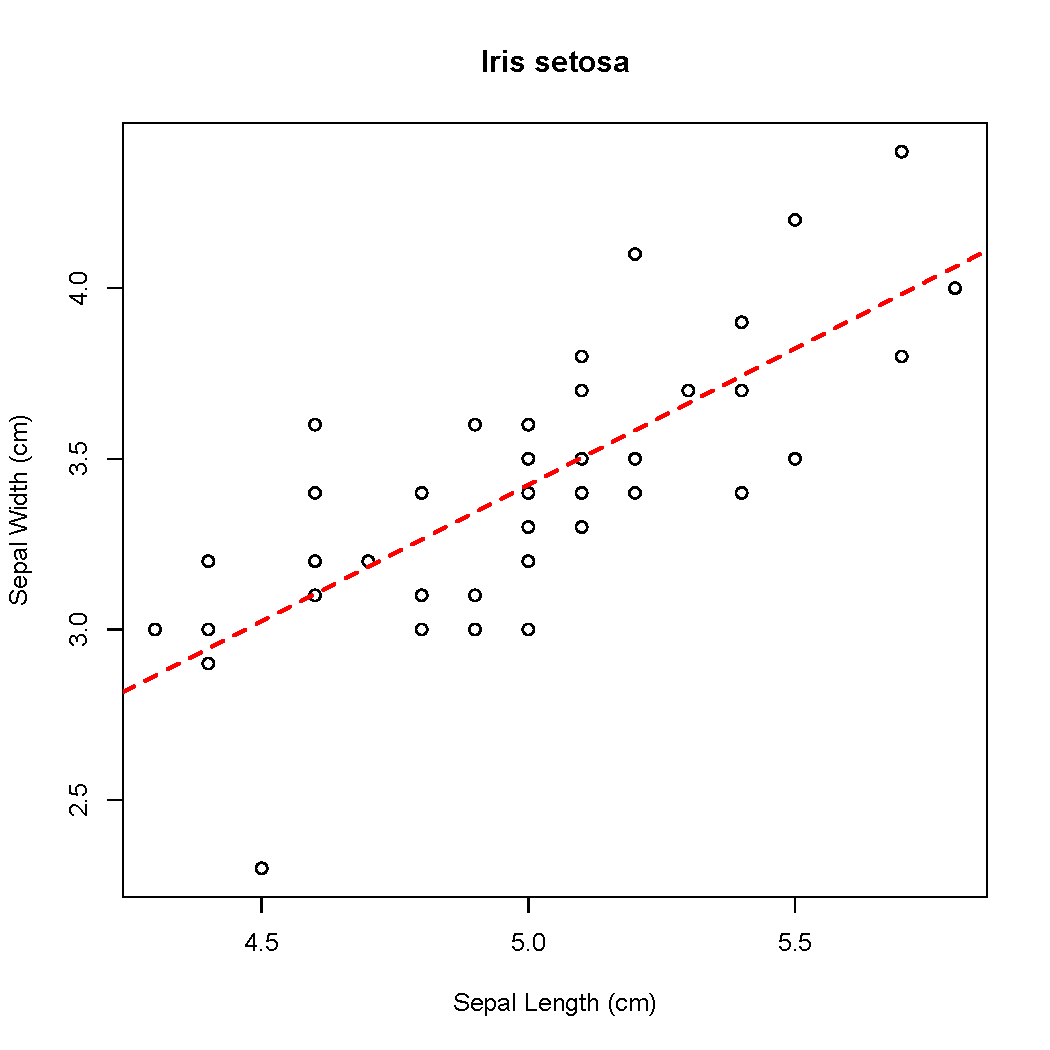
\includegraphics[width=0.5\columnwidth]{./figures/hands-on2/regression.pdf}
\caption{Linear regression of Sepal Width on Sepal Length for \Species{I.~setosa}.}
\end{figure}

\begin{assignment}
Write your own regression function (i.e.~your
code shouldn't refer to the built in regression functions) for mean
centered vectors in R. The function will take as it's input two vectors,
$\vec{x}$ and $\vec{y}$. The function should return:

\begin{enumerate}[1.]
\item
  a list containing the mean-centered versions of these vectors
\item
  the regression coefficient $b$ in the mean centered regression
  equation $\vec{\widehat{y}} = b\vec{x}$
\item
  the coefficient of determination, $R^2$
\end{enumerate}
Demonstrate your regression function by using it to carry out
regressions of Sepal.Length on Sepal.Width separately for the `versicolor'
and `virginica' specimens from the iris data set. Include plots in which you use the
\lstinline!plot()! and \lstinline!abline()! functions to illustrate your
calculated regression line. To test your function, compare your regression coefficients and coefficient of determination to the same values returned by the built in |lm()| function.

\end{assignment}



